---
title: Binary Search
date: 2018-05-22
author: Oliver Fleckenstein
---
\section{Searching Strategies}

    Searching for elements in a data structure is one of the fundamental problems for every computer scientist and programmer will encounter.
    Given an array $A$ of integers, consider the problem of determine if $x$ apprears in the array or not.

    \begin{figure}
        \centering
        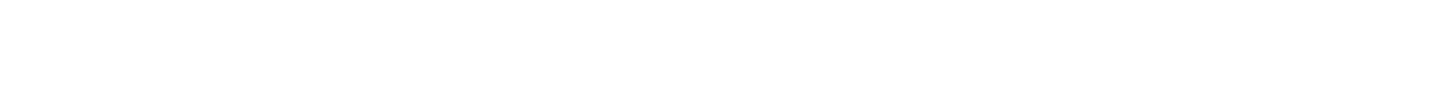
\includegraphics{/images/integer_array.png}
    \end{figure}

    A naive approach to this problem is to do a \emph{linear search}.
    That is to go through each of the elements one by one, checking if they are equal to $x$.
    It is easy to see that this approach will use linear time, $O(n)$, as in worst case the element is not in the array, and the algorithm will then look at each element in the array.

    \subsection{A better approach - Binary Search}

